\documentclass{standalone}
\usepackage{tikz}
\usetikzlibrary{positioning, shapes.misc}

\begin{document}

\begin{tikzpicture}

% Placeholder image
\node[inner sep=0, outer sep=0] (image) at (0,0) {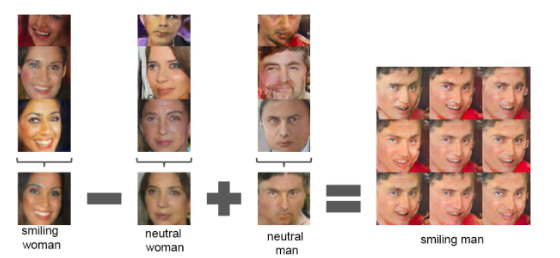
\includegraphics[width=15cm,height=6cm]{tikz/chapter9 - Arithmetics of GAN.png}};
\node[fill=white, xshift=-6.3cm, yshift=-2.52cm] {Smiling};
\node[fill=white, xshift=-6.3cm, yshift=-2.92cm] {Woman};
\node[fill=white, xshift=-3.1cm, yshift=-2.52cm] {Neutral};
\node[fill=white, xshift=-3.1cm, yshift=-2.92cm] {Woman};
\node[fill=white, xshift=0.1cm, yshift=-2.52cm] {Neutral};
\node[fill=white, xshift=0.1cm, yshift=-2.92cm] {Man};
\node[fill=white, xshift=4.6cm, yshift=-2.52cm, minimum width=5cm, minimum height=0.5cm] {};
\node[fill=white, xshift=4.6cm, yshift=-2.52cm] {Smiling};
\node[fill=white, xshift=4.6cm, yshift=-2.92cm] {Man};
\end{tikzpicture}

\end{document}